\documentclass[11pt]{article}

\usepackage[margin=0.85in]{geometry}
\usepackage{graphicx}
\usepackage{booktabs}
\usepackage{float}
\usepackage{caption}
\captionsetup{font=small,skip=4pt}
\usepackage{listings}
\usepackage{xcolor}
\usepackage[hidelinks]{hyperref}

\lstset{
  basicstyle=\ttfamily\footnotesize,
  breaklines=true,
  frame=single,
  showstringspaces=false,
}

\lstdefinestyle{cpp}{
  language=C++,
  basicstyle=\ttfamily\scriptsize,
  keywordstyle=\color{blue!70!black}\bfseries,
  commentstyle=\color{green!45!black}\itshape,
  stringstyle=\color{orange!80!black},
  emph={size_t,rrpv,victim,max_rrpv,distance},
  emphstyle=\color{purple!70!black},
  showstringspaces=false,
  breaklines=true,
  frame=single,
  rulecolor=\color{gray!55},
  columns=fullflexible,
  keepspaces=true,
  xleftmargin=2pt,
  aboveskip=4pt,
  belowskip=2pt,
}

\title{\textbf{E0245 HPCA Assignment 1}\\[0.5em]\Large Implementing the Hawkeye Cache Replacement Policy in ChampSim}
\author{
  Anirudh Gupta, Sr. No: 23600
}

\date{\today}

\begin{document}
\maketitle

\section{Introduction}

The goal of this assignment is to implement the Cache Replacement Policy(CRP) - Hawkeye from \textbf{Back to the Future: Leveraging Belady's Algorithm for Improved Cache Replacement}, with ChampSim simulator and evaluate its performance by measuring Cache Miss Rates(CMR) against the default LRU policy. We test the performance against 3 different associativities and 3 different datasets too. Beyond these I experimented around with different parameters and ideas, to see whether the chosen method/parameters are actually well chosen or not. These experiments are just to satisfy some curiosity. and patterns in data. I will be mentioning some of them below while discussing the my learnings.

GitHub Repository Link: \url{https://github.com/AnirudhG07/Champsim}, contains the code for the implementation of Hawkeye cache replacement, result files and plots inside \texttt{experiments/} directory with a README mentioning steps to reproduce the results.

\section{Learnings/Observations}

Top 3 learnings/observations while implementing this assignment are mentioned below. 

\subsection{Training Improve CMR}

LRU CRP even though widely used, shows lesser performance than the Hawkeye CRP. This is a not just a Hawkeye, but a general observation from other papers in different CS fields too, that any fixed heuristic based, static parameters based, and a non-learning based approach will always be outperformed by a learning based approach. That latter might need more time, resources, and data to train, but it usually outperforms the former, sometimes by even a significant margin. This is visible in our results too.

Concretely, Hawkeye replaces a fixed heuristic with a feedback loop. OPTgen reconstructs what Belady's optimal algorithm would have done over the recent access stream, which yields a ground-truth label for every reference: was this line worth keeping? That label is attributed back to the load instruction that brought the line in, and accumulated in a saturating counter indexed by that PC. At fill time the policy no longer guesses from recency alone --- it asks what this particular instruction's lines have historically been worth. LRU, by contrast, applies one rule to every line regardless of which instruction requested it, so a streaming load that never reuses its data is treated identically to a hot pointer dereference. The gain comes from exactly that distinction, which is why it is largest on workloads that mix access patterns and smallest on workloads that are uniformly streaming.

\subsection{Implementation based Learnings}

Here I talk about some insights and observations I made while implementing the Hawkeye CRP in the ChampSim simulator.

\subsubsection{Reusing the access sequence table}

Both OPTgen and the Hawkeye adapter need a per-set history of the last $8W$ accesses, but for different reasons. OPTgen stores the \emph{block\ address} accessed at each step, and scans backwards for a matching address to recover the usage interval; it never sees a PC, since its interface is \texttt{access(set\_idx, address)}. The adapter needs the \emph{PC} of the previous access to the same block, because OPTgen's verdict grades the access that loaded the line, not the one demanding it now.

My first implementation kept a second ring in \texttt{hawkeye.cc} holding both the block address and the PC, and scanned it independently --- duplicating OPTgen's address array and repeating the same backward walk twice per access. Since both rings are indexed by the same clock and cover the same window, this is redundant. Exposing two read-only accessors from OPTgen, \texttt{current\_time(set)} and \texttt{last\_distance(set)}, lets the adapter drop its address array entirely and keep only \texttt{pc\_seq}, indexed by OPTgen's clock. This removes roughly 2,MB of state, halves the per-access scanning, and makes clock drift between the two structures impossible. I verified the refactor is behaviour-preserving: the LLC miss rate was identical on both benchmarks before and after.

\subsubsection{Significance of \texttt{acces\_type::WRITE} in CRP} \label{sec:writeback}

Apart from just the logic of Hawkeye, champsim other CRP's used \texttt{acces\_type::WRITE} to deal with writebacks. That depends on the CRP and is different for different CRP's as it can be seen in \texttt{lru.cc}, \texttt{ship.cc}.
\textbf{What is \texttt{access\_type::WRITE}?} While scowering through the definitions, I found that \texttt{access\_type::WRITE} is not associated with any ip at all, rather it is used to mark a block evicted from higher level cache and written to lower level(LLC). Since we deal with LLC, we need to handle this case in our CRP too.  

In the function \texttt{update\_replacement\_state()}, we deal with a general behavior of the CRP, which for us means predict, train and update rrpv. For a cache block, if it is a writeback, we can't need to train the predictor since it is not associated with any ip. We also avoid searching through the access sequence history table, because that lookup
exists only to recover the PC to train with, and a writeback has none --- \texttt{cache.cc}
constructs the packet with \verb|writeback_packet.ip = champsim::address{}|. Feeding a
writeback to OPTgen would in fact be worse than useless: it is not a demand reference, yet
it would occupy a slot in the occupancy vector and shift every later timestamp, distorting
the usage intervals of the real accesses around it. Though for such a line, since it is a FILL in the cache block, the \texttt{replacement\_cache\_fill} function deals with it and we still need to update the rrpv of the block since we know the \texttt{set, way} for the block, and we can update the rrpv of the block between 0-7 or not set. However, since the block will replace an evicted line, it will be put in the cache with a rrpv having 7, which is equivalent to not setting the rrpv of the block. Logically it makes sense to keep it at 7 since the line since it is a writeback, it might not cache friendly and hence better of not to cache it. If it sees a hit on itself, we will update the rrpv of the block to 0, and it will be future tracked by the whole pipeline.

I tried setting the rrpv of the block to 0-7 and not-setting at all, and the results are as expected. It is better of not setting the rrpv of the block than marking it with a rrpv of 0-6 for potential usage in the future, this is confirmed in the experiments section \ref{sec:rrpv} in Figure~\ref{fig:writeback}, where we see that miss rates is linearly decreasing from 0-7 and CMR of 7 and none(not setting) is exactly same.

Hence dealing with \texttt{access\_type::WRITE} is important in the CRP, and we need to handle it properly.

\paragraph{P.S.} Coding this assignment by digging into different files like \texttt{cache.cc}, \texttt{lru.cc}, etc. made me realize that implementing a CRP is less complex than I thought. I always imagined it to be a 1000 lines of code, but it is quite cute, especially lru. Even though it is just a simulator, but still real world systems won't be that complicated either, hopefully. 

\subsection{Result Observations}

\subsubsection{Improvements of CMR with Associativity}

As the associativity of the cache increases, the CMR decreases. This is because with more ways, there are more blocks in each set. However notice that the reduction in CMR is not linear with associativity. This trend makes sense since associativity only removes \emph{conflict} misses, and those are largely exhausted by eight ways. Going from four to eight ways gives each set twice the room to hold competing lines, which eliminates most of the conflicts that a 4-way set cannot absorb. Beyond that, the misses that remain are capacity and compulsory misses, which more ways cannot fix --- the total LLC capacity is held fixed at 2,MB across the sweep, so increasing associativity only redistributes the same number of blocks into fewer, larger sets. The curve therefore flattens, and the benefit of a smarter replacement policy shrinks with it: with 16 candidates per set, even LRU usually has a reasonable line to evict, whereas at four ways a single bad eviction is far more costly.

\subsubsection{Observation of CRP on different datasets}

Across the three benchmarks the outcome tracks how much reuse there is to exploit. \texttt{456.hmmer} and \texttt{473.astar} improve by $2.79\%$ and $1.56\%$, while \texttt{429.mcf} regresses by $11.32\%$. The difference is based on workloads in different datasets. On \texttt{mcf} only $37\%$ of LLC references find a previous access to the same block inside OPTgen's $8W$ history window, against $60\%$ on \texttt{hmmer} and $78\%$ on \texttt{astar} (these results are self generated as explained in the Experiments section \ref{sec:dataset_patterns}). The predictor is therefore trained on far fewer samples, and its decisions are less reliable. The result is that Hawkeye's informed guesses are worse than LRU's uninformed ones, and the miss rate rises for \texttt{mcf}. This shows that the different workloads have different behavior and a CRP should be able to minimize the CRP overall on such workloads.


\section{Results}

\subsection{LLC Miss Rate versus Associativity}

\begin{figure}[H]
\centering
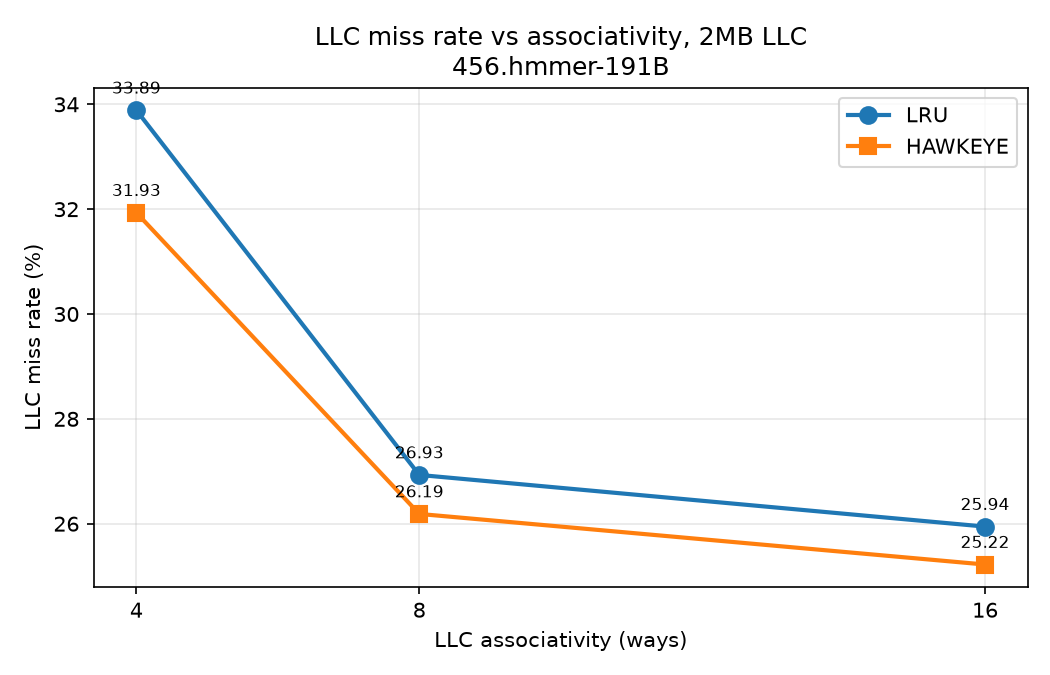
\includegraphics[width=0.51\textwidth]{../plot_1.png}
\caption{LLC miss rate versus LLC associativity on \texttt{456.hmmer-191B}, with total
LLC capacity held fixed at 2\,MB (64\,B lines) by scaling the set count inversely.
20\,M warmup / 50\,M simulated instructions. Lower is better.}
\label{fig:plot1}
\end{figure}

\begin{table}[H]
\centering\small
\begin{tabular}{rrrrr}
\toprule
Ways & Sets & LRU (\%) & Hawkeye (\%) & Reduction (\%) \\
\midrule
4  & 8192 & 33.89 & 31.93 & 5.77 \\
8  & 4096 & 26.93 & 26.19 & 2.76 \\
16 & 2048 & 25.94 & 25.22 & 2.79 \\
\bottomrule
\end{tabular}
\caption{LLC miss rate versus associativity on \texttt{456.hmmer-191B}.}
\label{tab:plot1}
\end{table}

Both policies improve sharply from four to eight ways and then flatten, confirming that
conflict misses dominate at low associativity and are largely exhausted by eight ways.
More interesting is that Hawkeye's \emph{advantage} over LRU is greatest where the cache
is most constrained: $5.77\%$ at four ways, against roughly $2.8\%$ at eight and sixteen.
With only four candidates per set a single poorly chosen eviction is expensive and there
is little slack to recover from it, so an informed decision is worth more. At sixteen ways
LRU almost always has a reasonable victim available on recency alone, and the margin for a
smarter policy narrows correspondingly. That the figures at eight and sixteen ways are
nearly identical suggests the misses which remain are capacity and compulsory misses,
which no replacement policy can remove.

\subsection{Miss-Rate Reduction across Benchmarks}

\begin{figure}[H]
\centering
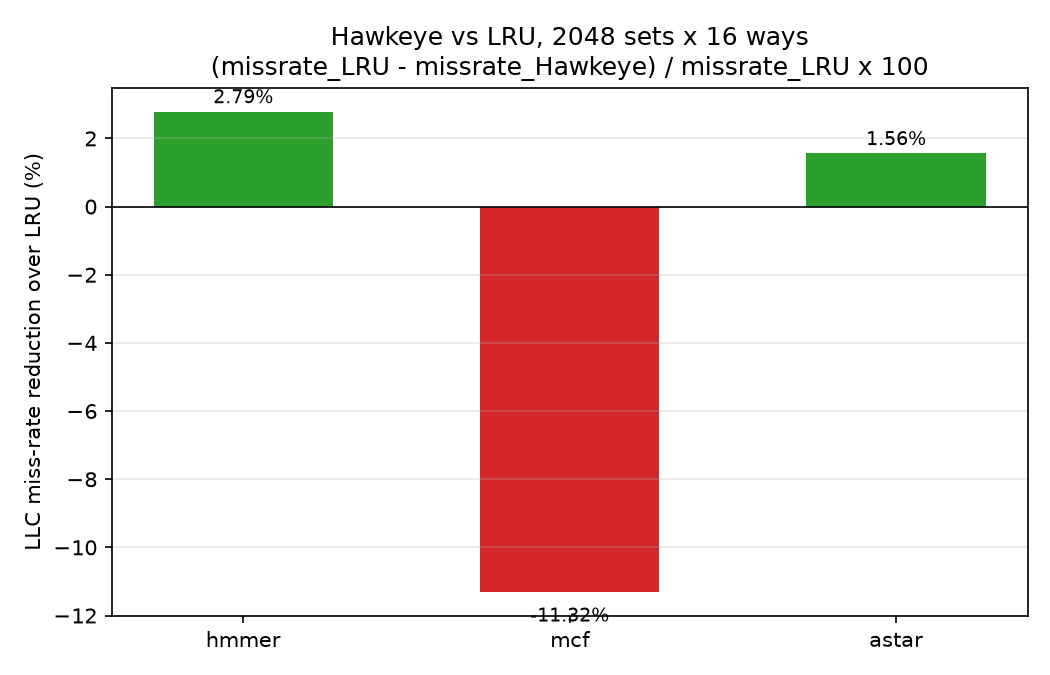
\includegraphics[width=0.58\textwidth]{../plot_2.png}
\caption{LLC miss-rate reduction over LRU for Hawkeye across three SPEC CPU2006
benchmarks at the default LLC geometry (2048 sets $\times$ 16 ways), computed as
$(\mathrm{missrate}_{\mathrm{LRU}} - \mathrm{missrate}_{\mathrm{Hawkeye}}) /
\mathrm{missrate}_{\mathrm{LRU}} \times 100$. Positive is better.}
\label{fig:plot2}
\end{figure}

\begin{table}[H]
\centering\small
\begin{tabular}{lrrr}
\toprule
Benchmark & LRU (\%) & Hawkeye (\%) & Reduction (\%) \\
\midrule
456.hmmer-191B & 25.94 & 25.22 & $2.79$   \\
429.mcf-22B    & 64.82 & 72.16 & $-11.32$ \\
473.astar-42B  & 19.63 & 19.33 & $1.56$   \\
\bottomrule
\end{tabular}
\caption{LLC miss rate at the default geometry (2048 sets, 16 ways).}
\label{tab:plot2}
\end{table}

\clearpage

\section{Experiments}

This section contains some experiments I did to see the effect of different parameters on the performance of the Hawkeye CRP and why.

\subsection{Effect of the Writeback Insertion RRPV} \label{sec:rrpv}

While implementing the Hawkeye CRP, usage of \texttt{access\_type::WRITE} is important to handle the writeback fills in the cache as shown in Figure~\ref{acc_type}. As discussed in section \ref{sec:writeback}, these writeback fills are not associated with any ip, but they still need to be updated in the rrpv(we have the block and set value). By logic mentioned previously, best value would be to have it at 7 or not set at all(should be by equivalent by construction). Hence to verify which value of rrpv is best, I did an experiment where I set the rrpv of the writeback fill to 0-7 and not set at all, and measured the miss rate reduction over LRU. The results are shown in Figure~\ref{fig:writeback} and Table~\ref{tab:writeback}.

\begin{lstlisting}[style=cpp,caption={Handling of \texttt{access\_type::WRITE} in \texttt{update\_replacement\_state()}.},label={acc_type}]
if (type == ACCESS_TYPE_WRITE) { /* for writeback hits */
  /* rrpv[set][way] = value; */ /* choose the appropriate RRPV value */
  return;
}
\end{lstlisting}

The results show that the best value of rrpv for writeback fills is 7 or not setting it at all, which is as expected.


\begin{figure}[H]
\centering
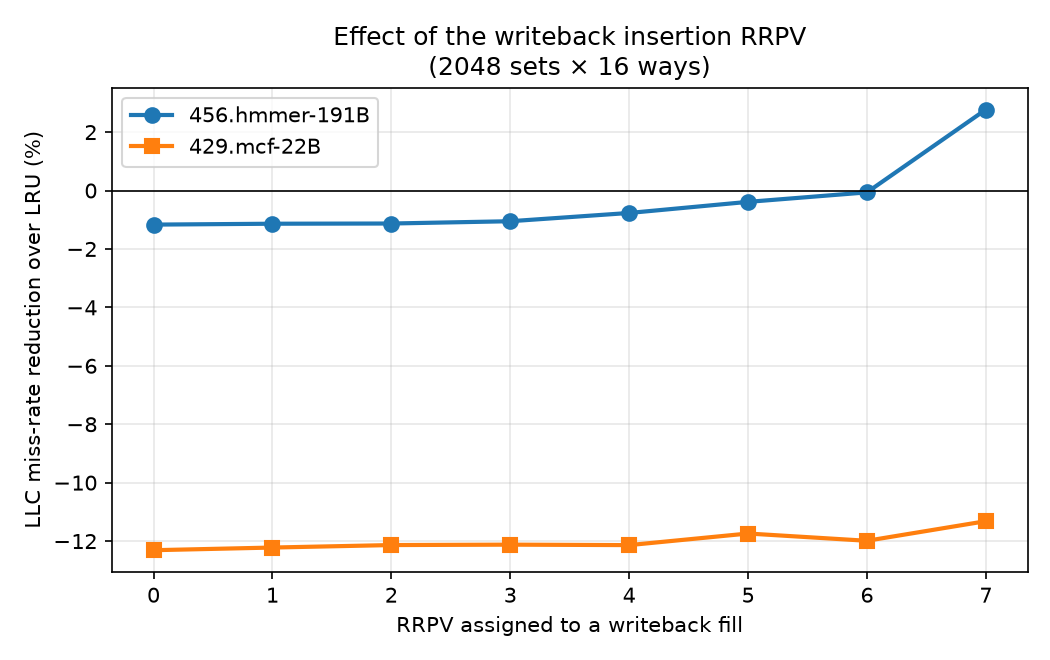
\includegraphics[width=\textwidth]{../plot_3.png}
\caption{LLC miss-rate reduction over LRU as a function of the RRPV assigned to a
writeback fill in \texttt{replacement\_cache\_fill}, for both \texttt{find\_victim}
variants. \texttt{none} denotes not setting the RRPV at all and letting the predictor
classify the writeback using its (absent) \texttt{ip}. Measured at the default LLC configs.}
\label{fig:writeback}
\end{figure}

\begin{table}[H]
\centering
\begin{tabular}{lrr}
\toprule
Writeback RRPV & 456.hmmer-191B & 429.mcf-22B \\
\midrule
0    & $-1.17$ & $-12.31$ \\
1    & $-1.14$ & $-12.22$ \\
2    & $-1.13$ & $-12.14$ \\
3    & $-1.05$ & $-12.12$ \\
4    & $-0.77$ & $-12.14$ \\
5    & $-0.39$ & $-11.74$ \\
6    & $-0.06$ & $-11.99$ \\
7    & $2.77$  & $-11.32$ \\
none & $2.77$  & $-11.32$ \\
\bottomrule
\end{tabular}
\caption{LLC miss-rate reduction over LRU (\%) for each writeback insertion RRPV,
using the assignment's \texttt{find\_victim}. Higher is better. The \texttt{none}
row --- not setting the RRPV at all --- is numerically identical to RRPV~7, and is
omitted from Figure~\ref{fig:writeback} for clarity.}
\label{tab:writeback}
\end{table}


\subsection{RRPV update, Paper vs Assignment}

The assignment mentions that, while finding the victim using the rrpv, we need to age all lines until we find a line with rrpv=7(or if previously present). Meanwhile the paper mentions that finding the value with maximum rrpv and evicting it is enough. The paper also mentions that a cache friendly line should never have rrpv = 7. Comparing the two methods theoretically, the paper's method should be better since it is not letting multiple cache friendly lines to be aged to 7. Once we start aging all lines, the victim will remain the same for that instruction, but for the future victims, we promotd a cache friendly line to 7 which would be evicted in the future. Hence the paper's method avoids such increments and lets only cache averse lines be evicted primarily, and only unless they donot exist that we evict a cache friendly line.

To test this hypothesis I made the two methods within rrpv's \texttt{find\_victim()} function and measured the miss rate reduction with each other. Figure~\ref{fig:lst-findvictim} shows the two methods. The results, as observable in Figure~\ref{fig:findvictim}, verify the hypothesis on
\texttt{456.hmmer} but not on \texttt{429.mcf}.

\begin{figure}[H]
\centering
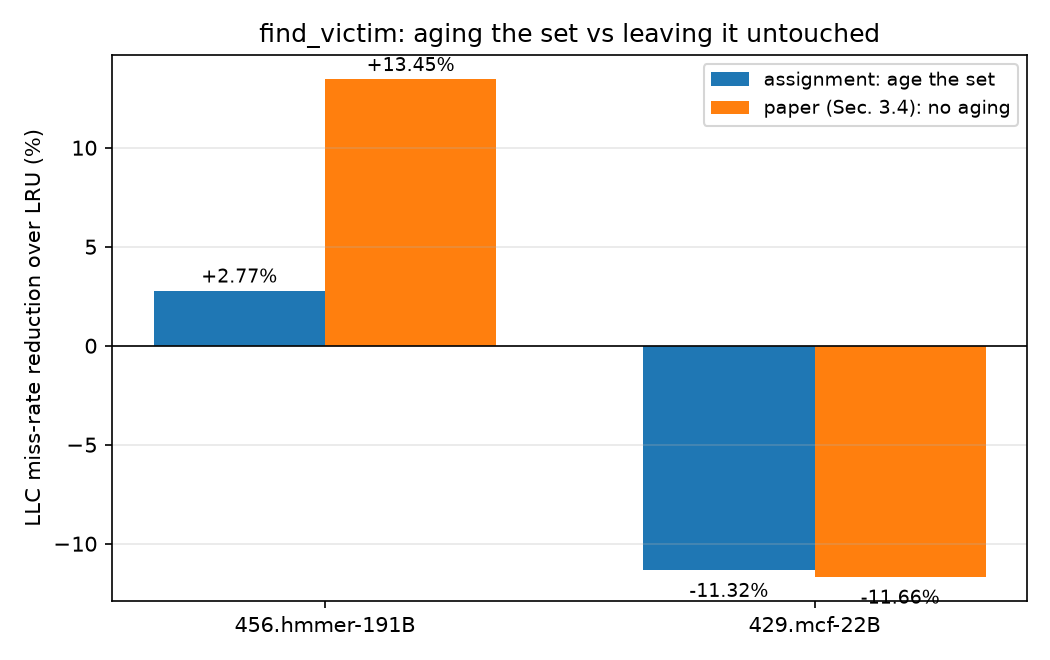
\includegraphics[width=0.75\textwidth]{../plot_4.png}
\caption{LLC miss-rate reduction over LRU for the two \texttt{find\_victim} variants of
Figure~\ref{lst:findvictim}, at the default LLC geometry (2048 sets $\times$ 16 ways).
Removing the aging step is worth almost five times the reduction on
\texttt{456.hmmer}, but makes no useful difference on \texttt{429.mcf}.}
\label{fig:findvictim}
\end{figure}


\begin{figure}[H]
\centering
\begin{minipage}[t]{0.48\textwidth}
\centering
\textbf{\small Assignment: age the set}
\begin{lstlisting}[style=cpp]
// find the way holding the maximum RRPV
int max_rrpv = rrpv[0];
size_t victim = 0;
for (size_t i = 1; i < rrpv.size(); i++) {
  if (rrpv[i] > max_rrpv) {
    max_rrpv = rrpv[i];
    victim = i;
  }
}

// age every line until the max reaches 7
const int distance = 7 - max_rrpv;
if (distance > 0) {
  for (size_t i = 0; i < rrpv.size(); i++) {
    rrpv[i] += distance;
  }
}

return victim;
\end{lstlisting}
\end{minipage}\hfill
\begin{minipage}[t]{0.48\textwidth}
\centering
\textbf{\small Paper (Sec. 3.4): no aging}
\begin{lstlisting}[style=cpp]
// find the way holding the maximum RRPV
int max_rrpv = rrpv[0];
size_t victim = 0;
for (size_t i = 1; i < rrpv.size(); i++) {
  if (rrpv[i] > max_rrpv) {
    max_rrpv = rrpv[i];
    victim = i;
  }
}

// the set is left untouched


return victim;
\end{lstlisting}
\end{minipage}
\caption{The two \texttt{find\_victim()} variants, showing only the part that differs.
Both walk the RRPV vector once and return the way holding the maximum, so they always
select the \emph{same} victim; they differ solely in whether the set is aged as a side
effect. The assignment's rule raises every RRPV by $7 - \max$, which promotes
cache-friendly lines to~7 and makes them indistinguishable from cache-averse ones on
subsequent evictions.}
\label{fig:lst-findvictim}
\end{figure}


\subsection{Understanding Dataset Patterns} \label{sec:dataset_patterns}

\texttt{429.mcf} was the one benchmark on which Hawkeye lost to LRU, and none of the design choices swept above accounted for it. To find out why, I temporarily added five counters to \texttt{struct hawkeye} and printed them once at the end of the run through ChampSim's \texttt{replacement\_final\_stats()} hook. Only the added lines are shown;
they were removed again before submission.

\begin{lstlisting}[style=cpp,caption={Counters added to \texttt{hawkeye} (additions only).},label=lst:diag]
// members of struct hawkeye
long diag_accesses = 0, diag_opt_hits = 0, diag_prev_found = 0;
long diag_fills = 0, diag_fills_friendly = 0;

// in update_replacement_state(), after d = optgen.last_distance(set)
diag_accesses   += 1;
diag_opt_hits   += optgen_hit ? 1 : 0;
diag_prev_found += (d > 0) ? 1 : 0;

// in replacement_cache_fill(), after the prediction is made
diag_fills          += 1;
diag_fills_friendly += _pred ? 1 : 0;

// ChampSim calls this once, after the simulation ends
void hawkeye::replacement_final_stats() {
  auto pct = [](long a, long b) { return b ? 100.0 * a / b : 0.0; };
  std::cout << "HAWKEYE_DIAG"
            << " opt_hit_rate="       << pct(diag_opt_hits,      diag_accesses)
            << " prev_found_rate="    << pct(diag_prev_found,    diag_accesses)
            << " friendly_fill_rate=" << pct(diag_fills_friendly, diag_fills) << "\n";
}
\end{lstlisting}

\begin{table}[H]
\centering\small
\begin{tabular}{lrrrr}
\toprule
Benchmark & OPT hit (\%) & Prev.\ found (\%) & Friendly fills (\%) & Reduction (\%) \\
\midrule
473.astar-42B  & 78.36 & 78.60 & 99.99 & $1.56$    \\
456.hmmer-191B & 58.22 & 60.49 & 97.75 & $2.79$    \\
429.mcf-22B    & 24.93 & 37.47 & 75.08 & $-11.32$  \\
\bottomrule
\end{tabular}
\caption{Policy-internal rates at the default LLC geometry. \emph{Prev.\ found} is the
fraction of references having an earlier access to the same block inside OPTgen's $8W$
history window.}
\label{tab:diag}
\end{table}

The three benchmarks order identically by \emph{prev.\ found} and by outcome. On \texttt{astar} and \texttt{hmmer} the OPT hit rate almost equals the prev.\ found rate($78.36$ against $78.60$, and $58.22$ against $60.49$), meaning that whenever a previous access lies inside the window it is nearly always an OPT hit --- OPTgen is answering from evidence. On \texttt{mcf} only $37\%$ of references have a previous access at all, and of those barely two thirds are hits, so the majority of references are labelled OPT misses by default rather than by observation. Those labels train the corresponding PCs negatively, the predictor classifies their lines cache-averse, and they are inserted at RRPV~7 and evicted almost immediately --- lines that LRU would have kept. \texttt{mcf} streams through a working set far larger than the 2\,MB LLC, so there is little reuse for any policy to capture, while Hawkeye still pays the cost of every misprediction. The regression is therefore a property of the access stream meeting a finite history window, not an implementation error.

\begin{center}
\Large ************
\end{center}

\end{document}
